\documentclass[12pt,a4paper]{article}
\usepackage[utf8]{inputenc}
\usepackage[utf8]{vietnam}
\usepackage{amsmath}
\usepackage{amsfonts}
\usepackage{amssymb}
\usepackage{pdflscape}
\usepackage{rotating}
\usepackage{xfrac}
\usepackage{booktabs}
\usepackage{indentfirst}
\usepackage[unicode,hidelinks=true]{hyperref}
\usepackage{graphicx}
\usepackage{subfig}
\usepackage{enumerate}
\usepackage{multicol}
\usepackage[left=1.5cm,right=2cm,top=1.5cm,bottom=2cm]{geometry}
\graphicspath{{images/}}
\usepackage[subpreambles=true]{standalone}
\usepackage{import}
\usepackage[labelfont={bf}, textfont={it}, skip=0pt]{caption}
\setlength{\belowcaptionskip}{-10pt}

\everymath{\displaystyle}
\renewcommand{\arraystretch}{1.5}
\renewcommand{\baselinestretch}{1.2}

\newcounter{exercise}[section]
\newenvironment{exercise}[1][]
    {\refstepcounter{exercise} \textbf{Bài tập~\thesection.\theexercise~}\rmfamily}{}

\newcounter{solution}[section]
\newenvironment{solution}[1][]
        {\refstepcounter{solution} \textbf{Bài giải~\thesection.\theexercise~}\rmfamily\\\par}{}

\newcommand{\fig}[1]{\textbf{Hình~#1}}
\newcommand{\pfm}[1]{\left({#1}\right)}
\newcommand{\pfs}[1]{\left[{#1}\right]}
\newcommand{\unit}[1]{~#1}

\title{\textbf{Bài tập Điều khiển quá trình \bigskip \\ Ôn tập thi cuối kỳ}}
% \author{Thực hiện: Thi Minh Nhựt \and Email: thiminhnhut@gmail.com}
\author{Thực hiện: \href{thiminhnhut@gmail.com}{Thi Minh Nhựt} -- Lê Thị Thu Ngân}
\date{Thời gian: \today}

\begin{document}

    \maketitle

    \tableofcontents

    \section{Phân tích hệ thống điều khiển phản hồi}
    \subsection{Xấp xỉ mô hình bậc cao theo phương pháp Skogestad (luật chia đôi)}
    Cho mô hình của đối tượng có dạng như sau:
    \begin{align*}
        G(s) = \dfrac{\displaystyle k \prod_{i=1}^m \left({-\tau_{zi} s + 1}\right)}{\displaystyle \prod_{j=1}^n \left({\tau_{pj} s + 1}\right)} e^{-\tau_0 s} \quad \textrm{ với } \tau_{p1} > \tau_{p2} > \tau_{p3} > \cdots
    \end{align*}

    \begin{itemize}
        \item Xấp xỉ về khâu quán tính bậc nhất có trễ với mô hình: $\tilde{G}(s) = \dfrac{k e^{-\theta s}}{\tau s + 1}$, trong đó:
            \begin{align*}
                \tau & = \tau_{p1} + \dfrac{\tau_{p2}}{2}; &
                \theta & = \tau_0 + \dfrac{\tau_{p2}}{2} + \sum_{j = 3}^n \tau_{pj} + \sum_{i = 1}^m \tau_{zi} \\
                & & & = \tau_0 + \dfrac{\tau_{p2}}{2} + \left({\tau_{p3} + \tau_{p4} + \cdots + \tau_{pn}}\right) + \left({\tau_{z1} + \tau_{z2} + \cdots + \tau_{zm}}\right)
            \end{align*}

        \item Xấp xỉ về khâu quán tính bậc hai có trễ với mô hình: $\tilde{G}(s) = \dfrac{k e^{-\theta s}}{\left({\tau_1 s + 1}\right) \left({\tau_2 s + 1}\right)}$, trong đó:
            \begin{align*}
                \tau_1 & = \tau_{p1}; & \tau_2 & = \tau_{p2} + \dfrac{\tau_{p3}}{2}; &
                \theta & = \tau_0 + \dfrac{\tau_{p3}}{2} + \sum_{j = 4}^n \tau_{pj} + \sum_{i = 1}^m \tau_{zi} \\
                & & & & & = \tau_0 + \dfrac{\tau_{p3}}{2} + \left({\tau_{p4} + \tau_{p5} + \cdots + \tau_{pn}}\right) + \left({\tau_{z1} + \tau_{z2} + \cdots + \tau_{zm}}\right)
                \end{align*}
    \end{itemize}

\subsection{Hàm truyền của bộ điều khiển PI và PID}
    \begin{itemize}
        \item Hàm truyền của bộ điều khiển PI cho khâu quán tính bậc nhất có dạng:
            \begin{align*}
                K(s) = K_P + \dfrac{K_I}{s} = K_P \left({1 + \dfrac{1}{T_I s}}\right)
            \end{align*}

        \item Hàm truyền của bộ điều khiển PID cho khâu quán tính bậc hai có dạng:
            \begin{align*}
                K(s) = K_P + \dfrac{K_I}{s} + K_D s = K_P \left({1 + \dfrac{1}{T_I s} + T_D s}\right)
            \end{align*}
    \end{itemize}

\subsection{Phương pháp xác định các thông số của bộ điều khiển PI và PID dựa trên mô hình mẫu}
\subsubsection{Phương pháp Haalman}
    \begin{itemize}
        \item Với khâu quán tính bậc nhất $\tilde{G}(s) = \dfrac{k e^{-\theta s}}{\tau s + 1}$ (mô hình FOPDT), sử dụng bộ điều khiển PI:
            \begin{align*}
                K(s) = K_P \left({1 + \dfrac{1}{T_I s}}\right) \quad \textrm{với} \quad K_P = \dfrac{2 \tau}{3 k \theta}; \quad T_I = \tau
            \end{align*}

        \item Với khâu quán tính bậc hai $\tilde{G}(s) = \dfrac{k e^{-\theta s}}{\left({\tau_1 s + 1}\right) \left({\tau_2 s + 1}\right)}$ (mô hình SOPDT), sử dụng bộ điều khiển PID:
            \begin{align*}
                K(s) = K_P \left({1 + \dfrac{1}{T_I s} + T_D s}\right) \quad \textrm{với} \quad K_P = \dfrac{2 \left({\tau_1 + \tau_2}\right)}{3 k \theta}; \quad T_I = \tau_1 + \tau_2; \quad T_D = \dfrac{\tau_1 \tau_2}{\tau_1 + \tau_2}
            \end{align*}
    \end{itemize}

\subsubsection{Phương pháp tổng hợp trực tiếp (Direct Synthesis -- DS)}
    \begin{itemize}
        \item Với khâu quán tính bậc nhất $\tilde{G}(s) = \dfrac{k e^{-\theta s}}{\tau s + 1}$ (mô hình FOPDT), sử dụng bộ điều khiển PI:
        \begin{align*}
            K(s) = K_P \left({1 + \dfrac{1}{T_I s}}\right) \quad \textrm{với} \quad K_P = \dfrac{\tau}{k\left({\tau_c + \theta}\right)}; \quad T_I = \tau
        \end{align*}

        với $\tau_c$ là hằng số thời gian quán tính.

        \item Với khâu quán tính bậc hai $\tilde{G}(s) = \dfrac{k e^{-\theta s}}{\left({\tau_1 s + 1}\right) \left({\tau_2 s + 1}\right)}$ (mô hình SOPDT), sử dụng bộ điều khiển PID:
            \begin{align*}
                K(s) = K_P \left({1 + \dfrac{1}{T_I s} + T_D s}\right) \quad \textrm{với} \quad K_P = \dfrac{\tau_1 + \tau_2}{k\left({\tau_c + \theta}\right)}; \quad T_I = \tau_1 + \tau_2; \quad T_D = \dfrac{\tau_1 \tau_2}{\tau_1 + \tau_2}
            \end{align*}

        với $\tau_c$ là hằng số thời gian quán tính.
    \end{itemize}

\subsubsection{Bảng tổng hợp xác định thông số của bộ điều khiển PI, PID theo phương pháp Haalman và phương pháp tổng hợp trực tiếp}
    \begin{table}[htp]
        \begin{center}
            \begin{tabular}{llll}
                \toprule
                \multicolumn{2}{c}{Khâu quán tính bậc nhất (FOPDT)} & \multicolumn{2}{c}{Khâu quán tính bậc hai (SOPDT)} \\
                \multicolumn{2}{c}{$\tilde{G}(s) = \dfrac{k e^{-\theta s}}{\tau s + 1}$} & \multicolumn{2}{c}{$\tilde{G}(s) = \dfrac{k e^{-\theta s}}{\left({\tau_1 s + 1}\right) \left({\tau_2 s + 1}\right)}$} \\
                \multicolumn{2}{c}{$K_{PI}(s) = K_P \left({1 + \dfrac{1}{T_I s}}\right)$} & \multicolumn{2}{c}{$K_{PID}(s) = K_P \left({1 + \dfrac{1}{T_I s} + T_D s}\right)$} \\
                \midrule
                Phương pháp Haalman & Phương pháp DS & Phương pháp Haalman & Phương pháp DS \\
                \midrule
                $K_P = \dfrac{2 \tau}{3 k \theta}$ & $K_P = \dfrac{\tau}{k\left({\tau_c + \theta}\right)}$  & $K_P = \dfrac{2 \left({\tau_1 + \tau_2}\right)}{3 k \theta}$ & $K_P = \dfrac{\tau_1 + \tau_2}{k\left({\tau_c + \theta}\right)}$ \\
                $T_I = \tau$ & $T_I = \tau$ & $T_I = \tau_1 + \tau_2$ & $T_I = \tau_1 + \tau_2$ \\
                & & $T_D = \dfrac{\tau_1 \tau_2}{\tau_1 + \tau_2}$ & $T_D = \dfrac{\tau_1 \tau_2}{\tau_1 + \tau_2}$ \\
                \bottomrule
            \end{tabular}
        \end{center}
        \caption{Xác định các thông số của bộ điều khiển PI, PID theo phương pháp Haalman và phương pháp tổng hợp trực tiếp}
    \end{table}



    \documentclass[12pt,a4paper]{article}
\usepackage[utf8]{inputenc}
\usepackage[utf8]{vietnam}
\usepackage{amsmath}
\usepackage{amsfonts}
\usepackage{amssymb}
\usepackage{xfrac}
\usepackage{booktabs}
\usepackage{indentfirst}
\usepackage{graphicx}
\usepackage{subfig}
\usepackage{enumerate}
\usepackage[left=2cm,right=2cm,top=2cm,bottom=2cm]{geometry}
\graphicspath{{images/}}
\usepackage[subpreambles=true]{standalone}
\usepackage{import}

\everymath{\displaystyle}
\renewcommand{\arraystretch}{1.5}
\renewcommand{\baselinestretch}{1.2}

\newcounter{exercise}[section]
\newenvironment{exercise}[1][]
    {\refstepcounter{exercise} \textbf{Bài tập~\thesection.\theexercise~}\rmfamily}{}

\newcounter{solution}[section]
\newenvironment{solution}[1][]
        {\refstepcounter{solution} \textbf{Bài giải~\thesection.\theexercise~}\rmfamily\\\par}{}

\title{\textbf{Bài tập Điều khiển quá trình \bigskip \\ Chủ đề Chỉnh định bộ điều khiển PID}}
\author{Sưu tầm: Thi Minh Nhựt \and Email: thiminhnhut@gmail.com}
\date{Thời gian: \today}

\begin{document}

    \maketitle

    \tableofcontents

    \subsection{Xấp xỉ mô hình bậc cao theo phương pháp Skogestad (luật chia đôi)}
    Cho mô hình của đối tượng có dạng như sau:
    \begin{align*}
        G(s) = \dfrac{\displaystyle k \prod_{i=1}^m \left({-\tau_{zi} s + 1}\right)}{\displaystyle \prod_{j=1}^n \left({\tau_{pj} s + 1}\right)} e^{-\tau_0 s} \quad \textrm{ với } \tau_{p1} > \tau_{p2} > \tau_{p3} > \cdots
    \end{align*}

    \begin{itemize}
        \item Xấp xỉ về khâu quán tính bậc nhất có trễ với mô hình: $\tilde{G}(s) = \dfrac{k e^{-\theta s}}{\tau s + 1}$, trong đó:
            \begin{align*}
                \tau & = \tau_{p1} + \dfrac{\tau_{p2}}{2}; &
                \theta & = \tau_0 + \dfrac{\tau_{p2}}{2} + \sum_{j = 3}^n \tau_{pj} + \sum_{i = 1}^m \tau_{zi} \\
                & & & = \tau_0 + \dfrac{\tau_{p2}}{2} + \left({\tau_{p3} + \tau_{p4} + \cdots + \tau_{pn}}\right) + \left({\tau_{z1} + \tau_{z2} + \cdots + \tau_{zm}}\right)
            \end{align*}

        \item Xấp xỉ về khâu quán tính bậc hai có trễ với mô hình: $\tilde{G}(s) = \dfrac{k e^{-\theta s}}{\left({\tau_1 s + 1}\right) \left({\tau_2 s + 1}\right)}$, trong đó:
            \begin{align*}
                \tau_1 & = \tau_{p1}; & \tau_2 & = \tau_{p2} + \dfrac{\tau_{p3}}{2}; &
                \theta & = \tau_0 + \dfrac{\tau_{p3}}{2} + \sum_{j = 4}^n \tau_{pj} + \sum_{i = 1}^m \tau_{zi} \\
                & & & & & = \tau_0 + \dfrac{\tau_{p3}}{2} + \left({\tau_{p4} + \tau_{p5} + \cdots + \tau_{pn}}\right) + \left({\tau_{z1} + \tau_{z2} + \cdots + \tau_{zm}}\right)
                \end{align*}
    \end{itemize}

\subsection{Hàm truyền của bộ điều khiển PI và PID}
    \begin{itemize}
        \item Hàm truyền của bộ điều khiển PI cho khâu quán tính bậc nhất có dạng:
            \begin{align*}
                K(s) = K_P + \dfrac{K_I}{s} = K_P \left({1 + \dfrac{1}{T_I s}}\right)
            \end{align*}

        \item Hàm truyền của bộ điều khiển PID cho khâu quán tính bậc hai có dạng:
            \begin{align*}
                K(s) = K_P + \dfrac{K_I}{s} + K_D s = K_P \left({1 + \dfrac{1}{T_I s} + T_D s}\right)
            \end{align*}
    \end{itemize}

\subsection{Phương pháp xác định các thông số của bộ điều khiển PI và PID dựa trên mô hình mẫu}
\subsubsection{Phương pháp Haalman}
    \begin{itemize}
        \item Với khâu quán tính bậc nhất $\tilde{G}(s) = \dfrac{k e^{-\theta s}}{\tau s + 1}$ (mô hình FOPDT), sử dụng bộ điều khiển PI:
            \begin{align*}
                K(s) = K_P \left({1 + \dfrac{1}{T_I s}}\right) \quad \textrm{với} \quad K_P = \dfrac{2 \tau}{3 k \theta}; \quad T_I = \tau
            \end{align*}

        \item Với khâu quán tính bậc hai $\tilde{G}(s) = \dfrac{k e^{-\theta s}}{\left({\tau_1 s + 1}\right) \left({\tau_2 s + 1}\right)}$ (mô hình SOPDT), sử dụng bộ điều khiển PID:
            \begin{align*}
                K(s) = K_P \left({1 + \dfrac{1}{T_I s} + T_D s}\right) \quad \textrm{với} \quad K_P = \dfrac{2 \left({\tau_1 + \tau_2}\right)}{3 k \theta}; \quad T_I = \tau_1 + \tau_2; \quad T_D = \dfrac{\tau_1 \tau_2}{\tau_1 + \tau_2}
            \end{align*}
    \end{itemize}

\subsubsection{Phương pháp tổng hợp trực tiếp (Direct Synthesis -- DS)}
    \begin{itemize}
        \item Với khâu quán tính bậc nhất $\tilde{G}(s) = \dfrac{k e^{-\theta s}}{\tau s + 1}$ (mô hình FOPDT), sử dụng bộ điều khiển PI:
        \begin{align*}
            K(s) = K_P \left({1 + \dfrac{1}{T_I s}}\right) \quad \textrm{với} \quad K_P = \dfrac{\tau}{k\left({\tau_c + \theta}\right)}; \quad T_I = \tau
        \end{align*}

        với $\tau_c$ là hằng số thời gian quán tính.

        \item Với khâu quán tính bậc hai $\tilde{G}(s) = \dfrac{k e^{-\theta s}}{\left({\tau_1 s + 1}\right) \left({\tau_2 s + 1}\right)}$ (mô hình SOPDT), sử dụng bộ điều khiển PID:
            \begin{align*}
                K(s) = K_P \left({1 + \dfrac{1}{T_I s} + T_D s}\right) \quad \textrm{với} \quad K_P = \dfrac{\tau_1 + \tau_2}{k\left({\tau_c + \theta}\right)}; \quad T_I = \tau_1 + \tau_2; \quad T_D = \dfrac{\tau_1 \tau_2}{\tau_1 + \tau_2}
            \end{align*}

        với $\tau_c$ là hằng số thời gian quán tính.
    \end{itemize}

\subsubsection{Bảng tổng hợp xác định thông số của bộ điều khiển PI, PID theo phương pháp Haalman và phương pháp tổng hợp trực tiếp}
    \begin{table}[htp]
        \begin{center}
            \begin{tabular}{llll}
                \toprule
                \multicolumn{2}{c}{Khâu quán tính bậc nhất (FOPDT)} & \multicolumn{2}{c}{Khâu quán tính bậc hai (SOPDT)} \\
                \multicolumn{2}{c}{$\tilde{G}(s) = \dfrac{k e^{-\theta s}}{\tau s + 1}$} & \multicolumn{2}{c}{$\tilde{G}(s) = \dfrac{k e^{-\theta s}}{\left({\tau_1 s + 1}\right) \left({\tau_2 s + 1}\right)}$} \\
                \multicolumn{2}{c}{$K_{PI}(s) = K_P \left({1 + \dfrac{1}{T_I s}}\right)$} & \multicolumn{2}{c}{$K_{PID}(s) = K_P \left({1 + \dfrac{1}{T_I s} + T_D s}\right)$} \\
                \midrule
                Phương pháp Haalman & Phương pháp DS & Phương pháp Haalman & Phương pháp DS \\
                \midrule
                $K_P = \dfrac{2 \tau}{3 k \theta}$ & $K_P = \dfrac{\tau}{k\left({\tau_c + \theta}\right)}$  & $K_P = \dfrac{2 \left({\tau_1 + \tau_2}\right)}{3 k \theta}$ & $K_P = \dfrac{\tau_1 + \tau_2}{k\left({\tau_c + \theta}\right)}$ \\
                $T_I = \tau$ & $T_I = \tau$ & $T_I = \tau_1 + \tau_2$ & $T_I = \tau_1 + \tau_2$ \\
                & & $T_D = \dfrac{\tau_1 \tau_2}{\tau_1 + \tau_2}$ & $T_D = \dfrac{\tau_1 \tau_2}{\tau_1 + \tau_2}$ \\
                \bottomrule
            \end{tabular}
        \end{center}
        \caption{Xác định các thông số của bộ điều khiển PI, PID theo phương pháp Haalman và phương pháp tổng hợp trực tiếp}
    \end{table}


    \section{Bài tập áp dụng}

    \begin{exercise}
    Cho một thiết bị trao đổi nhiệt với hàm truyền từ tín hiệu điều khiển van dòng mang nhiệt và tín hiệu đo nhiệt độ ra của dòng quá trình là:
        \begin{align*}
            G(s) = \dfrac{0.75e^{-1.2s}}{(30s + 1)(5s + 1)(2s+1)}
        \end{align*}
    \begin{enumerate}
        \item Xấp xỉ hàm truyền theo quy tắc Skogestad:
            \begin{enumerate}
                \item Xấp xỉ hàm truyền $G(s)$ về dạng bậc nhất có trễ sử dụng quy tắc Skogestad.
                \item Xấp xỉ hàm truyền $G(s)$ về dạng bậc hai có trễ sử dụng quy tắc Skogestad.
            \end{enumerate}

        \item Thiết kế bộ điều khiển sử dụng phương pháp Haalman:
            \begin{enumerate}
                \item Thiết kế bộ điều khiển PI sử dụng phương pháp Haalman.
                \item Thiết kế bộ điều khiển PID sử dụng phương pháp Haalman.
            \end{enumerate}

        \item Thiết kế bộ điều khiển sử dụng phương pháp tổng hợp trực tiếp Direct Synthesis -- DS:
            \begin{enumerate}
                \item Thiết kế bộ điều khiển PI sử dụng phương pháp tổng hợp trực tiếp Direct Synthesis, biết hằng số thời gian của hệ kín là $\tau_c = 3.17$.

                \item Thiết kế bộ điều khiển PID sử dụng phương pháp tổng hợp trực tiếp Direct Synthesis, biết hằng số thời gian của hệ kín là $\tau_c = 3.17$.
            \end{enumerate}
    \end{enumerate}
\end{exercise}

\begin{solution}
    Ta có hàm truyền $G(s) = \dfrac{0.75e^{-1.21s}}{(30s + 1)(5s + 1)(2s+1)}$, nên:
        \begin{align*}
            k = 0.75; \quad \tau_{p1} = 30; \tau_{p2} = 5; \tau_{p3} = 2; \quad \tau_{0} = 1.21
        \end{align*}
    \begin{enumerate}
        \item \textbf{Xấp xỉ hàm truyền theo quy tắc Skogestad:}
            \begin{enumerate}
                \item Xấp xỉ hàm truyền $G(s)$ về dạng bậc nhất có trễ sử dụng quy tắc Skogestad.
                    \begin{align*}
                        & \left\{\begin{array}{l}
                            \tau = \tau_{p1} + \dfrac{\tau_{p2}}{2} = 30 + \dfrac{5}{2} = 32.5 \\
                            \theta = \tau_0 + \left({\dfrac{\tau_{p2}}{2} + \tau_{p3}}\right) + 0= 1.21 + \left({\dfrac{5}{2} + 2}\right) + 0 = 5.71
                        \end{array}\right. \\
                        \Longrightarrow &
                        \tilde{G}(s) = \dfrac{k e^{-\theta s}}{\tau s + 1} = \dfrac{0.75e^{-5.71s}}{32.5s + 1}
                    \end{align*}
                \item Xấp xỉ hàm truyền $G(s)$ về dạng bậc hai có trễ sử dụng quy tắc Skogestad.
                    \begin{align*}
                        & \left\{\begin{array}{l}
                            \tau_1 = \tau_{p1} = 30\\
                            \tau_2 = \tau_{p2} + \dfrac{\tau_{p3}}{2} = 5 + \dfrac{2}{2} = 6 \\
                            \theta = \tau_0 + 0 + 0 = 1.21 + 0 + 0 = 1.21
                        \end{array}\right. \\
                        \Longrightarrow &
                        \tilde{G}(s) = \dfrac{k e^{-\theta s}}{\left({\tau_1 s + 1}\right) \left({\tau_2 s + 1}\right)} = \dfrac{0.75 e^{-1.21s}}{\left({30s + 1}\right) \left({6s + 1}\right)}
                    \end{align*}
            \end{enumerate}

        \item \textbf{Thiết kế bộ điều khiển sử dụng phương pháp Haalman:}
            \begin{enumerate}
                \item Thiết kế bộ điều khiển PI sử dụng phương pháp Haalman.
                    \begin{itemize}
                        \item Ta có: $\tilde{G}(s) = \dfrac{0.75e^{-5.71s}}{32.5s + 1}$, suy ra: $k = 0.75; \theta = 5.71; \tau = 32.5$
                        \item Tính giá trị các thông số $K_P$ và $K_I$:
                            \begin{align*}
                                \left\{\begin{array}{l}
                                    K_P = \dfrac{2 \tau}{3 k \theta} = \dfrac{2 \times 32.5}{3 \times 0.75 \times 5.71} = 5.06\\
                                    T_I = \tau = 32.5
                                \end{array}\right.
                            \end{align*}
                        \item Kết luận: $K(s) = K_P \left({1 + \dfrac{1}{T_I s}}\right) = 5.06 \left({1 + \dfrac{1}{32.5 s}}\right)$
                    \end{itemize}
                \item Thiết kế bộ điều khiển PID sử dụng phương pháp Haalman.
                    \begin{itemize}
                        \item Ta có: $\tilde{G}(s) = \dfrac{0.75 e^{-1.21 s}}{\left({30s + 1}\right) \left({6s + 1}\right)}$, suy ra: $k = 0.75; \theta = 1.21; \tau_1 = 30; \tau_2 = 6$
                        \item Tính giá trị các thông số $K_P$ và $K_I$:
                            \begin{align*}
                                \left\{\begin{array}{l}
                                    K_P = \dfrac{2 \left({\tau_1 + \tau_2}\right)}{3 k \theta} = \dfrac{2 \left({30 + 6}\right)}{3 \times 0.75 \times 1.21} = 26.45 \\
                                    T_I = \tau_1 + \tau_2 = 30 + 6 = 36 \\
                                    T_D = \dfrac{\tau_1 \tau_2}{\tau_1 + \tau_2} = \dfrac{30 \times 6}{30 + 6} = 5
                                \end{array}\right.
                            \end{align*}
                        \item Kết luận: $K(s) = K_P \left({1 + \dfrac{1}{T_I s} + T_D s}\right) = 26.45 \left({1 + \dfrac{1}{36s} + 5s}\right)$
                    \end{itemize}
            \end{enumerate}

        \item \textbf{Thiết kế bộ điều khiển sử dụng phương pháp tổng hợp trực tiếp Direct Synthesis -- DS:}
        \begin{enumerate}
            \item Thiết kế bộ điều khiển PI sử dụng phương pháp tổng hợp trực tiếp Direct Synthesis, biết hằng số thời gian của hệ kín là $\tau_c = 3.17$.
                \begin{itemize}
                    \item Ta có: $\tilde{G}(s) = \dfrac{0.75e^{-5.71s}}{32.5s + 1}$, suy ra: $k = 0.75; \theta = 5.71; \tau = 32.5$
                    \item Tính giá trị các thông số $K_P$, $K_I$ và $T_D$:
                        \begin{align*}
                            \left\{\begin{array}{l}
                                K_P = \dfrac{\tau}{k\left({\tau_c + \theta}\right)} = \dfrac{32.5}{0.75 \times \left({3.17 + 5.71}\right)} = 4.88\\
                                T_I = \tau = 32.5
                            \end{array}\right.
                        \end{align*}
                    \item Kết luận: $K(s) = K_P \left({1 + \dfrac{1}{T_I s}}\right) = 4.88 \left({1 + \dfrac{1}{32.5 s}}\right)$
                \end{itemize}

            \item Thiết kế bộ điều khiển PID sử dụng phương pháp tổng hợp trực tiếp Direct Synthesis, biết hằng số thời gian của hệ kín là $\tau_c = 3.17$.
                \begin{itemize}
                    \item Ta có: $\tilde{G}(s) = \dfrac{0.75 e^{-1.21 s}}{\left({30s + 1}\right) \left({6s + 1}\right)}$, suy ra: $k = 0.75; \theta = 1.21; \tau_1 = 30; \tau_2 = 6$
                    \item Tính giá trị các thông số $K_P$, $K_I$ và $T_D$:
                        \begin{align*}
                            \left\{\begin{array}{l}
                                K_P = \dfrac{\tau_1 + \tau_2}{k\left({\tau_c + \theta}\right)} = \dfrac{30 + 6}{0.75 \times \left({3.17 + 1.21}\right)} = 10.96\\
                                T_I = \tau_1 + \tau_2 = 30 + 6 = 36\\
                                T_D = \dfrac{\tau_1 \tau_2}{\tau_1 + \tau_2} = \dfrac{30 \times 6}{30 + 6} = 5
                            \end{array}\right.
                        \end{align*}
                    \item Kết luận: $K(s) = K_P \left({1 + \dfrac{1}{T_I s} + T_D s}\right) = 10.96 \left({1 + \dfrac{1}{36s} + 5s}\right)$
                \end{itemize}
        \end{enumerate}
    \end{enumerate}
\end{solution}

    \begin{exercise}
    Một quá trình bao gồm cả cảm biến và van điều khiển có thể được mô hình hoá bởi hàm truyền trong các trường hợp sau:
        \begin{align*}
            G(s) & = \dfrac{0.5e^{-6s}}{(10s + 1)(8s + 1)(3s+1)(s+1)} \\
            G(s) & = \dfrac{1}{(s + 1)(0.2s + 1)(0.04s+1)(0.08s+1)} \\
            G(s) & = \dfrac{100(-0.1s + 1)}{(5s + 1)(3s + 1)(0.04s+1)(0.5s+1)} \\
            G(s) & = \dfrac{100(1 - s) e^{-s}}{(12s + 1)(3s + 1)(0.2s+1)(0.05s+1)} \\
            G(s) & = \dfrac{2(s + 0.5)(3s + 1) e^{-5s}}{(s + 2)(s + 1)(6s + 1)} \\
            G(s) & = \dfrac{2(-6s^2 + s + 1)e^{3s}}{(s + 2)(s + 1)(12s^2 + 17s + 6)}
        \end{align*}

    Thực hiện các yêu cầu bên dưới cho từng hàm truyền $G(s)$.

    \begin{enumerate}
        \item Xấp xỉ hàm truyền theo quy tắc Skogestad:
            \begin{enumerate}
                \item Xấp xỉ hàm truyền $G(s)$ về dạng bậc nhất có trễ sử dụng quy tắc Skogestad.
                \item Xấp xỉ hàm truyền $G(s)$ về dạng bậc hai có trễ sử dụng quy tắc Skogestad.
            \end{enumerate}

        \item Thiết kế bộ điều khiển sử dụng phương pháp Haalman:
            \begin{enumerate}
                \item Thiết kế bộ điều khiển PI sử dụng phương pháp Haalman.
                \item Thiết kế bộ điều khiển PID sử dụng phương pháp Haalman.
            \end{enumerate}

        \item Thiết kế bộ điều khiển sử dụng phương pháp tổng hợp trực tiếp Direct Synthesis -- DS:
            \begin{enumerate}
                \item Thiết kế bộ điều khiển PI sử dụng phương pháp tổng hợp trực tiếp Direct Synthesis, biết hằng số thời gian của hệ kín là $\tau_c = 0.51$.

                \item Thiết kế bộ điều khiển PID sử dụng phương pháp tổng hợp trực tiếp Direct Synthesis, biết hằng số thời gian của hệ kín là $\tau_c = 0.51$.
            \end{enumerate}
    \end{enumerate}
\end{exercise}

    \begin{exercise}
    Một quá trình bao gồm cả cảm biến và van điều khiển có thể được mô hình hoá bởi hàm truyền bậc 4 như sau:
        \begin{align*}
            G(s) = \dfrac{1}{(s + 1)(0.2s + 1)(0.04s+1)(0.08s+1)}
        \end{align*}
    \begin{enumerate}
        \item Xấp xỉ hàm truyền theo quy tắc Skogestad:
            \begin{enumerate}
                \item Xấp xỉ hàm truyền $G(s)$ về dạng bậc nhất có trễ sử dụng quy tắc Skogestad.
                \item Xấp xỉ hàm truyền $G(s)$ về dạng bậc hai có trễ sử dụng quy tắc Skogestad.
            \end{enumerate}

        \item Thiết kế bộ điều khiển sử dụng phương pháp Haalman:
            \begin{enumerate}
                \item Thiết kế bộ điều khiển PI sử dụng phương pháp Haalman.
                \item Thiết kế bộ điều khiển PID sử dụng phương pháp Haalman.
            \end{enumerate}

        \item Thiết kế bộ điều khiển sử dụng phương pháp tổng hợp trực tiếp Direct Synthesis -- DS:
            \begin{enumerate}
                \item Thiết kế bộ điều khiển PI sử dụng phương pháp tổng hợp trực tiếp Direct Synthesis, biết hằng số thời gian của hệ kín là $\tau_c = 0.51$.

                \item Thiết kế bộ điều khiển PID sử dụng phương pháp tổng hợp trực tiếp Direct Synthesis, biết hằng số thời gian của hệ kín là $\tau_c = 0.51$.
            \end{enumerate}
    \end{enumerate}
\end{exercise}

    \begin{exercise}
    Cho hệ thống như hình \ref{baitap1-1binhchua}: Biết lưu lượng ra $F_2$ tỉ lệ với chiều cao chất lỏng theo công thức $F_2 = R.h^{\sfrac{4}{3}}$ với $R$ là hằng số. Tiết diện của bồn chứa là $A$.
    \begin{figure}[htp]
        \begin{center}
            \subimport{../mohinhoalythuyet/images/}{baitap1-1binhchua.tex}
        \end{center}
        \caption{Hệ thống 1 bình chứa} \label{baitap1-1binhchua}
    \end{figure}

    \begin{enumerate}
        \item Xác định các biến vào, biến ra, biến điều khiển, biến cần điều khiển và biến nhiễu.
        \item Viết phương trình động học cho mức chất lỏng trong bồn chứa.
        \item Tuyến tính hóa phương trình xây dựng được xung quanh vị trí cân bằng dựa trên phương pháp khai triển Taylor.
        \item Xác định hàm truyền $G(s) = \dfrac{H(s)}{F_1(s)}$
        \item Thiết kế bộ điều khiển PI sử dụng phương pháp tổng hợp trực tiếp Direct Synthesis, biết hằng số thời gian của hệ kín là $\tau_c = 0.5$.
    \end{enumerate}
\end{exercise}



\end{document}


    \section{Bài tập Mô hình hóa lý thuyết và Thiết kế điều khiển}
    \subsection{Bài tập về thiết bị khuấy trộn liên tục}
\subsubsection{Mô hình về thiết bị khuấy trộn liên tục}
    \begin{figure}[htp]
        \begin{center}
            \subfloat[Mô hình 1 \label{Fig:binhchuachatlong-khuaytron-mohinh1}]
                {
                    \subimport{section/mohinhhoalythuyet/images/}{binhchuachatlong-khuaytron-mohinh1.tex}
                }
            \subfloat[Mô hình 2 \label{Fig:binhchuachatlong-khuaytron-mohinh2}]
                {
                    \subimport{section/mohinhhoalythuyet/images/}{binhchuachatlong-khuaytron-mohinh2.tex}
                }
            % \subfloat[Mô hình 3 \label{Fig:binhchuachatlong-khuaytron-mohinh3}]
            %     {
            %         \subimport{section/mohinhhoalythuyet/images/}{binhchuachatlong-khuaytron-mohinh3.tex}
            %     }
        \end{center}
        \caption{Các mô hình về thiết bị khuấy trộn liên tục} \label{Fig:binhchuachatlong-khuaytron}
    \end{figure}

\subparagraph{Các đại lượng trên mô hình}
    \begin{itemize}
		\item $w_1, w_2$: Lưu lượng khối lượng nguyên liệu của hai dòng nguyên liệu $\pfm{kg/s}$ hoặc $\pfm{kg/\text{\textit{phút}}}$.
		\item $x_1, x_2$: Thành phần của 2 dòng nguyên liệu.
		\item $w$: Lưu lượng khối lượng dòng sản phẩm ra $\pfm{kg/s}$ hoặc $\pfm{kg/\text{\textit{phút}}}$.
		\item $x$: Thành phần của sản phẩm ra.
		\item $h$: Mức chất lỏng trong bình $\pfm{m}$.
	\end{itemize}

\subparagraph{Mô tả quá trình} Hai dòng nguyên liệu có thành phần chất $A$ lần lượt là $x_1$ và $x_2$ được đưa vào thiết bị khuấy trộn, tạo ra một dòng sản phẩm có nồng độ $x$ theo yêu cầu. Lưu lượng dòng nguyên liệu được điều khiển qua các van. Quá trình pha chế được hỗ trợ bởi một hệ thống khuấy trộn gắn động cơ.

\subsubsection{Xác định các biến quá trình}
    \begin{itemize}
        \item Mô hình trong \fig{\ref{Fig:binhchuachatlong-khuaytron-mohinh1}}:
            \begin{center}
                \begin{tabular}{l|l}
                    Biến vào: $x_1, x_2$ và $w, w_1, w_2$ & Biến điều khiển: $w_1,w_2$ \\ \hline
                    Biến ra: $x,h$ & Biến cần điều khiển: $x,h$\\ \hline
                    & Biến nhiễu: $x_1, x_2$ và $w$
                \end{tabular}
            \end{center}

        \item Mô hình trong \fig{\ref{Fig:binhchuachatlong-khuaytron-mohinh2}}:
            \begin{center}
                \begin{tabular}{l|l}
                    Biến vào: $x_1, x_2$ và $w, w_1, w_2$ & Biến điều khiển: $w, w_1$ \\ \hline
                    Biến ra: $x,h$ & Biến cần điều khiển: $x,h$\\ \hline
                    & Biến nhiễu: $x_1, x_2$ và $w_2$
                \end{tabular}
            \end{center}
    \end{itemize}

\subsubsection{Xây dựng phương trình toán học}
    \begin{itemize}
        \item Giả thiết:
            \begin{itemize}
                \item Bỏ qua trễ do vận chuyển.
                \item Quá trình khuấy trộn được xem là lý tưởng, chất lỏng đồng nhất tại mọi vị trí trong thiết bị.
                \item Khối lượng riêng của hỗn hợp trong thiết bị được coi là thay đổi không đáng kể.
            \end{itemize}
        \item Công thức tính thể tích $V = Ah$ với $A$ là tiết diện của bình chứa.
        \item Áp dụng phương trình cân bằng vật chất:
            \begin{align*}
                \rho \dfrac{dV}{dt} = w_1 + w_2 - w \Longleftrightarrow \rho \dfrac{d\pfm{Ah}}{dt} = w_1 + w_2 - w \Longleftrightarrow \dfrac{dh}{dt} = \dfrac{1}{\rho A} \pfm{w_1 + w_2 - w}
            \end{align*}
        \item Phương trình cân bằng thành phần:
            \begin{align*}
                \rho \dfrac{d\pfm{Vx}}{dt} = w_1x_1 + w_2x_2 - wx
            \end{align*}
        \item Khai triển đạo hàm riêng cho vế trái, ta có phương trình:
            \begin{align*}
                & \rho V \dfrac{dx}{dt} + \rho x \dfrac{dV}{dt} = w_1x_1 + w_2x_2 - wx\\
                \Longleftrightarrow~ & \rho V \dfrac{dx}{dt} + x \pfm{w_1 + w_2 - w} = w_1x_1 + w_2x_2 - wx\\
                \Longleftrightarrow~ & \rho V \dfrac{dx}{dt} = w_1x_1 + w_2x_2 - \pfm{w_1 + w_2}x\\
                \Longleftrightarrow~ & \dfrac{dx}{dt} = \dfrac{1}{\rho V} \left[{w_1x_1 + w_2x_2 - \pfm{w_1 + w_2}x}\right]\\
                \Longleftrightarrow~ & \dfrac{dx}{dt} = \dfrac{1}{\rho A h} \left[{w_1x_1 + w_2x_2 - \pfm{w_1 + w_2}x}\right]
            \end{align*}
        \item Kết luận, mô hình toán của hệ thống là:
            \begin{align*}
                \left\{\begin{array}{l}
                    \dfrac{dh}{dt}  = \dfrac{1}{\rho A} \pfm{w_1 + w_2 - w}\\
                    \dfrac{dx}{dt}  = \dfrac{1}{\rho A h} \left[{w_1x_1 + w_2x_2 - \pfm{w_1 + w_2}x}\right]
                \end{array}\right.
            \end{align*}
    \end{itemize}

\subsubsection{Tuyến tính hóa phương trình quanh điểm làm việc cân bằng}
    \begin{itemize}
        \item Đặt: $h = \overline{h} + \Delta h$; $x = \overline{x} + \Delta x$; $w_1 = \overline{w}_1 + \Delta w_1$; $w_2 = \overline{w}_2 + \Delta w_2$; $w = \overline{w} + \Delta w$; $x_1 = \overline{x}_1 + \Delta x_1$; $x_2 = \overline{x}_2 + \Delta x_2$.
        \item Tại điểm làm việc cân bằng $(\overline{h}, \overline{x}, \overline{x}_1, \overline{x}_2, \overline{w}_1, \overline{w}_2, \overline{w})$, ta có:
            \begin{align*}
                \left\{\begin{array}{l}
                    \dfrac{dh}{dt}  = \dfrac{1}{\rho A} \pfm{\overline{w}_1 + \overline{w}_2 - \overline{w}} = 0 \\
                    \dfrac{dx}{dt}  = \dfrac{1}{\rho A \overline{h}} \left[{\overline{w}_1 \overline{x}_1 + \overline{w}_2 \overline{x}_2 - \pfm{\overline{w}_1 + \overline{w}_2}\overline{x}}\right] = 0
                \end{array}\right.
                \Longleftrightarrow
                \left\{\begin{array}{l}
                     \overline{w}_1 + \overline{w}_2 = \overline{w} \\
                    \overline{w}_1\overline{x}_1 + \overline{w}_2\overline{x}_2 - \pfm{\overline{w}_1 + \overline{w}_2}\overline{x} = 0
                \end{array}\right.
            \end{align*}
        \item Ta có: $\dfrac{dh}{dt}  = \dfrac{1}{\rho A} \pfm{w_1 + w_2 - w}$ đã tuyến tính hóa, nên:
            \begin{align*}
                \dot{h} = \Delta \dot{h} = \dfrac{1}{\rho A} \pfm{\Delta w_1 + \Delta w_2 - \Delta w}
            \end{align*}
        \item Khai triển Taylor cho $f(h, x, x_1, x_2, w_1, w_2, w) = \dfrac{dx}{dt}  = \dfrac{1}{\rho A h} \left[{w_1x_1 + w_2x_2 - \pfm{w_1 + w_2}x}\right]$ tại điểm làm việc cân bằng $(\overline{h}, \overline{x}, \overline{x}_1, \overline{x}_2, \overline{w}_1, \overline{w}_2, \overline{w})$, ta có:
            \begin{align*}
                \dot{x} = \Delta \dot{x} = & \underbrace{f(\overline{h}, \overline{x}, \overline{x}_1, \overline{x}_2, \overline{w}_1, \overline{w}_2, \overline{w})}_{0} + \dfrac{df}{dh}\Delta h + \dfrac{df}{dx}\Delta x + \dfrac{df}{dx_1}\Delta x_1 + \dfrac{df}{dx_2}\Delta x_2 + \dfrac{df}{dw_1}\Delta w_1 \\
                & + \dfrac{df}{dw_2}\Delta w_2 + \dfrac{df}{dw}\Delta w \\
                = & \dfrac{-1}{\rho A \overline{h}^2} \underbrace{\left[{\overline{w}_1 \overline{x}_1 + \overline{w}_2 \overline{x}_2 - \pfm{\overline{w}_1 + \overline{w}_2}\overline{x}}\right]}_{0} \Delta h + \dfrac{-1}{\rho A \overline{h}} \underbrace{\pfm{\overline{w}_1 + \overline{w}_2}}_{\overline{w}} \Delta x + \dfrac{\overline{w}_1}{\rho A \overline{h}} \Delta x_1 + \dfrac{\overline{w}_2}{\rho A \overline{h}} \Delta x_2 \\
                & + \dfrac{\overline{x}_1 - \overline{x}}{\rho A \overline{h}} \Delta w_1 + \dfrac{\overline{x}_2 - \overline{x}}{\rho A \overline{h}} \Delta w_2 + 0\\
                = & - \dfrac{\overline{w}}{\rho A \overline{h}} \Delta x + \dfrac{\overline{w}_1}{\rho A \overline{h}} \Delta x_1 + \dfrac{\overline{w}_2}{\rho A \overline{h}} \Delta x_2 + \dfrac{\overline{x}_1 - \overline{x}}{\rho A \overline{h}} \Delta w_1 + \dfrac{\overline{x}_2 - \overline{x}}{\rho A \overline{h}} \Delta w_2
            \end{align*}
        \item Kết luận, mô hình tuyến tính hóa theo khai triển Taylor có dạng:
            \begin{align*}
                \left\{\begin{array}{l}
                    \Delta \dot{h} = \dfrac{1}{\rho A} \pfm{\Delta w_1 + \Delta w_2 - \Delta w}\\
                    \Delta \dot{x} = - \dfrac{\overline{w}}{\rho A \overline{h}} \Delta x + \dfrac{\overline{w}_1}{\rho A \overline{h}} \Delta x_1 + \dfrac{\overline{w}_2}{\rho A \overline{h}} \Delta x_2 + \dfrac{\overline{x}_1 - \overline{x}}{\rho A \overline{h}} \Delta w_1 + \dfrac{\overline{x}_2 - \overline{x}}{\rho A \overline{h}} \Delta w_2
                \end{array}\right.
            \end{align*}
    \end{itemize}

\subsubsection{Xây dựng hàm truyền và vẽ sơ đồ khối mô tả quá trình}
    \begin{itemize}
        \item Ta có $\Delta \dot{h} = \dfrac{1}{\rho A} \pfm{\Delta w_1 + \Delta w_2 - \Delta w}$, khai triển Laplace:
            \begin{align*}
                & s \Delta H(s) = \dfrac{1}{\rho A} \left[{\Delta W_1(s) + \Delta W_2(s) - \Delta W(s)}\right]\\
                \Longleftrightarrow & \Delta H(s) = \dfrac{1}{\rho As} \Delta W_1(s) + \dfrac{1}{\rho As} \Delta W_2(s) - \dfrac{1}{\rho As} \Delta W(s)
            \end{align*}

        \item Đặt $k_{wh} = \dfrac{1}{\rho A}$, ta có: $\Delta H(s) = \dfrac{k_{wh}}{s} \Delta W_1(s) + \dfrac{k_{wh}}{s} \Delta W_2(s) - \dfrac{k_{wh}}{s} \Delta W(s)$
        \item Ta có $\Delta \dot{x} = - \dfrac{\overline{w}}{\rho A \overline{h}} \Delta x + \dfrac{\overline{w}_1}{\rho A \overline{h}} \Delta x_1 + \dfrac{\overline{w}_2}{\rho A \overline{h}} \Delta x_2 + \dfrac{\overline{x}_1 - \overline{x}}{\rho A \overline{h}} \Delta w_1 + \dfrac{\overline{x}_2 - \overline{x}}{\rho A \overline{h}} \Delta w_2$, khai triển Laplace:
            \begin{align*}
                & s X(s) = - \dfrac{\overline{w}}{\rho A \overline{h}} \Delta X(s) + \dfrac{\overline{w}_1}{\rho A \overline{h}} \Delta X_1(s) + \dfrac{\overline{w}_2}{\rho A \overline{h}} \Delta X_2(s) + \dfrac{\overline{x}_1 - \overline{x}}{\rho A \overline{h}} \Delta W_1(s) + \dfrac{\overline{x}_2 - \overline{x}}{\rho A \overline{h}} \Delta W_2(s) \\
                \Longleftrightarrow & \rho A \overline{h} s X(s) + \overline{w} \Delta X(s) = \overline{w}_1 \Delta X_1(s) + \overline{w}_2 \Delta X_2(s) + \pfm{\overline{x}_1 - \overline{x}} \Delta W_1(s) + \pfm{\overline{x}_2 - \overline{x}} \Delta W_2(s)\\
                \Longleftrightarrow & \pfm{\dfrac{\rho A \overline{h}}{\overline{w}}s + 1}\Delta X(s) = \dfrac{\overline{w}_1}{\overline{w}} \Delta X_1(s) + \dfrac{\overline{w}_2}{\overline{w}} \Delta X_2(s) + \dfrac{\overline{x}_1 - \overline{x}}{\overline{w}} \Delta W_1(s) + \dfrac{\overline{x}_2 - \overline{x}}{\overline{w}} \Delta W_2(s)
            \end{align*}
        \item Đặt $\tau = \dfrac{\rho A \overline{h}}{\overline{w}}$; $k_{x1x} = \dfrac{\overline{w}_1}{\overline{w}}$; $k_{x2x} = \dfrac{\overline{w}_2}{\overline{w}}$; $k_{w1x} = \dfrac{\overline{x}_1 - \overline{x}}{\overline{w}}$; $k_{w2x} = \dfrac{\overline{x}_2 - \overline{x}}{\overline{w}}$, ta có:
            \begin{align*}
                & \pfm{\tau s + 1}\Delta X(s) = k_{x1x} \Delta X_1(s) + k_{x2x} \Delta X_2(s) + k_{w1x} \Delta W_1(s) + k_{w2x} \Delta W_2(s) \\
                \Longleftrightarrow & \Delta X(s) = \dfrac{k_{x1x}}{\tau s + 1} \Delta X_1(s) + \dfrac{k_{x2x}}{\tau s + 1} \Delta X_2(s) + \dfrac{k_{w1x}}{\tau s + 1} \Delta W_1(s) + \dfrac{k_{w2x}}{\tau s + 1} \Delta W_2(s)
            \end{align*}
        \item Kết luận:
            \begin{align*}
                \left\{\begin{array}{l}
                    \Delta H(s) = \dfrac{k_{wh}}{s} \Delta W_1(s) + \dfrac{k_{wh}}{s} \Delta W_2(s) - \dfrac{k_{wh}}{s} \Delta W(s)\\
                    \Delta X(s) = \dfrac{k_{x1x}}{\tau s + 1} \Delta X_1(s) + \dfrac{k_{x2x}}{\tau s + 1} \Delta X_2(s) + \dfrac{k_{w1x}}{\tau s + 1} \Delta W_1(s) + \dfrac{k_{w2x}}{\tau s + 1} \Delta W_2(s)\\
                    k_{wh} = \dfrac{1}{\rho A}; \tau = \dfrac{\rho A \overline{h}}{\overline{w}}; k_{x1x} = \dfrac{\overline{w}_1}{\overline{w}}; k_{x2x} = \dfrac{\overline{w}_2}{\overline{w}}; k_{w1x} = \dfrac{\overline{x}_1 - \overline{x}}{\overline{w}}; k_{w2x} = \dfrac{\overline{x}_2 - \overline{x}}{\overline{w}}
                \end{array}\right.
            \end{align*}

        \item Ta có các hàm truyền mô tả hệ thống như sau:
            \begin{align*}
                \left\{\begin{array}{l}
                    \dfrac{H(s)}{W_1(s)} = \dfrac{k_{wh}}{s}; \dfrac{H(s)}{W_2(s)} = \dfrac{k_{wh}}{s}; \dfrac{H(s)}{W(s)} = -\dfrac{k_{wh}}{s}; \dfrac{H(s)}{X_1(s)} = 0; \dfrac{H(s)}{X_2(s)} = 0\\
                    \dfrac{X(s)}{W_1(s)} = \dfrac{k_{w1x}}{\tau s + 1}; \dfrac{X(s)}{W_2(s)} = \dfrac{k_{w2x}}{\tau s + 1}; \dfrac{X(s)}{X_1(s)} = \dfrac{k_{x1x}}{\tau s + 1}; \dfrac{X(s)}{X_2(s)} = \dfrac{k_{x2x}}{\tau s + 1}; \dfrac{X(s)}{W(s)} = 0 \\
                    k_{wh} = \dfrac{1}{\rho A}; \tau = \dfrac{\rho A \overline{h}}{\overline{w}}; k_{x1x} = \dfrac{\overline{w}_1}{\overline{w}}; k_{x2x} = \dfrac{\overline{w}_2}{\overline{w}}; k_{w1x} = \dfrac{\overline{x}_1 - \overline{x}}{\overline{w}}; k_{w2x} = \dfrac{\overline{x}_2 - \overline{x}}{\overline{w}}
                \end{array}\right.
            \end{align*}

    \item Giả thiết: thiết bị khuấy trộn liên tục có tiết diện đều $A = 0.8\unit{m^2}$ và khối lượng riêng của chất lỏng $\rho = 1.25 \unit{kg/\textrm{lít}} = 1.25 \times 10^3 \unit{kg/m^3}$, được vận hành với các thông số tại điểm làm việc cân bằng như sau: $\overline{w}_2 = 200 \unit{kg/\textrm{phút}}$, $\overline{x} = 0.4$, $\overline{x}_1 = 0.8$, $\overline{x}_2 = 0.2$, $\overline{h} = 1 \unit{m}$.
        \begin{itemize}
            \item Từ điều kiện cân bằng, ta có: $\left\{\begin{array}{l}\overline{w}_1 + \overline{w}_2 = \overline{w}\\ \overline{w}_1\overline{x}_1 + \overline{w}_2\overline{x}_2 - \pfm{\overline{w}_1 + \overline{w}_2}\overline{x} = 0\end{array}\right.$, thay các giá trị vào, ta được:
                \begin{align*}
                    & \left\{\begin{array}{l}
                         \overline{w}_1 + 200 = \overline{w}\\
                        \overline{w}_1 \times 0.8 + 200 \times 0.2 - \pfm{\overline{w}_1 + 200}\times 0.4 = 0
                    \end{array}\right.
                    \Longleftrightarrow
                    \left\{\begin{array}{l}
                         \overline{w}_1 + 200 = \overline{w}\\
                        0.8\overline{w}_1 + 40 - 0.4\overline{w}_1 - 80 = 0
                    \end{array}\right.\\
                    \Longleftrightarrow &
                    \left\{\begin{array}{l}
                         \overline{w}_1 + 200 = \overline{w}\\
                        0.4\overline{w}_1 - 40 = 0
                    \end{array}\right.
                    \Longleftrightarrow
                    \left\{\begin{array}{l}
                         \overline{w} = 100 + 200 \\
                        \overline{w}_1 = 100
                    \end{array}\right.
                    \Longleftrightarrow
                    \left\{\begin{array}{l}
                         \overline{w} = 300 \unit{kg/\textrm{phút}}\\
                        \overline{w}_1 = 100 \unit{kg/\textrm{phút}}
                    \end{array}\right.
                \end{align*}

            \item Khi đó, ta có:
                \begin{align*}
                    \left\{\begin{array}{l}
                        k_{wh} = \dfrac{1}{\rho A} = \dfrac{1}{1.25 \times 10^3 \times 0.8} = 0.001 \unit{m/kg}; \\
                        \tau = \dfrac{\rho A \overline{h}}{\overline{w}} = \dfrac{1.25 \times 10^3 \times 0.8 \times 1}{300} = \dfrac{10}{3} \unit{\textrm{phút}}; \\
                        k_{x1x} = \dfrac{\overline{w}_1}{\overline{w}} = \dfrac{100}{300} = \dfrac{1}{3}; \qquad k_{x2x} = \dfrac{\overline{w}_2}{\overline{w}} = \dfrac{200}{300} = \dfrac{2}{3}; \\
                        k_{w1x} = \dfrac{\overline{x}_1 - \overline{x}}{\overline{w}} = \dfrac{0.8 - 0.4}{300} = \dfrac{1}{750} \unit{\textrm{phút}/kg}; \\
                        k_{w2x} = \dfrac{\overline{x}_2 - \overline{x}}{\overline{w}} = \dfrac{0.2 - 0.4}{300} = \dfrac{1}{1500} \unit{\textrm{phút}/kg}
                    \end{array}\right.
                \end{align*}
        \end{itemize}

        \item Với quá trình được mô tả trên \fig{\ref{Fig:binhchuachatlong-khuaytron-mohinh1}}:
            \begin{itemize}
                \item Đặt: $y = \left[\begin{array}{c}\Delta h \\ \Delta x \end{array}\right]; \qquad u = \left[\begin{array}{c}\Delta w_1 \\ \Delta w_2 \end{array}\right]; \qquad d = \left[\begin{array}{c}\Delta x_1 \\ \Delta x_2 \\ \Delta w \end{array}\right]$
                \item Suy ra: $y(s) = G_p u(s) + G_d d(s)$, với các ma trận $G_p$ và $G_d$ như sau:
                    \begin{align*}
                        G_p = \left[\begin{array}{cc}\dfrac{k_{wh}}{s} & \dfrac{k_{wh}}{s} \\ \dfrac{k_{w1x}}{\tau s + 1} & \dfrac{k_{w2x}}{\tau s + 1} \end{array}\right]; \qquad G_d = \left[\begin{array}{ccc}0 & 0 & -\dfrac{k_{wh}}{s} \\ \dfrac{k_{x1x}}{\tau s + 1} & \dfrac{k_{x2x}}{\tau s + 1} & 0 \end{array}\right]
                    \end{align*}
                \item Sơ đồ khối: \fig{\ref{Fig:binhchuachatlong-khuaytron-mohinh1-sodokhoi}}.
                    \begin{figure}[!htp]
                        \begin{center}
                            \subimport{section/mohinhhoalythuyet/images/}{binhchuachatlong-khuaytron-mohinh1-sodokhoi.tex}
                        \end{center}
                        \caption{Sơ đồ khối cho mô hình 1} \label{Fig:binhchuachatlong-khuaytron-mohinh1-sodokhoi}
                    \end{figure}
            \end{itemize}

        \item Với quá trình được mô tả trên \fig{\ref{Fig:binhchuachatlong-khuaytron-mohinh2}}:
            \begin{itemize}
                \item Đặt: $y = \left[\begin{array}{c}\Delta h \\ \Delta x \end{array}\right]; \qquad u = \left[\begin{array}{c}\Delta w_1 \\ \Delta w \end{array}\right]; \qquad d = \left[\begin{array}{c}\Delta x_1 \\ \Delta x_2 \\ \Delta w_2 \end{array}\right]$
                \item Suy ra: $y(s) = G_p u(s) + G_d d(s)$, với các ma trận $G_p$ và $G_d$ như sau:
                    \begin{align*}
                        G_p = \left[\begin{array}{cc}\dfrac{k_{wh}}{s} & -\dfrac{k_{wh}}{s} \\ \dfrac{k_{w1x}}{\tau s + 1} & 0\end{array}\right]; \qquad G_d = \left[\begin{array}{ccc}0 & 0 & \dfrac{k_{wh}}{s} \\ \dfrac{k_{x1x}}{\tau s + 1} & \dfrac{k_{x2x}}{\tau s + 1} & 0 \end{array}\right]
                    \end{align*}
                \item Sơ đồ khối: \fig{\ref{Fig:binhchuachatlong-khuaytron-mohinh2-sodokhoi}}.
                    \begin{figure}[!htp]
                        \begin{center}
                            \subimport{section/mohinhhoalythuyet/images/}{binhchuachatlong-khuaytron-mohinh2-sodokhoi.tex}
                        \end{center}
                        \caption{Sơ đồ khối cho mô hình 2} \label{Fig:binhchuachatlong-khuaytron-mohinh2-sodokhoi}
                    \end{figure}
            \end{itemize}
    \end{itemize}

\subsubsection{Vẽ sơ đồ khối cho cấu trúc điều khiển phản hồi}
    \begin{landscape}
        \begin{figure}[htp]
            \begin{center}
                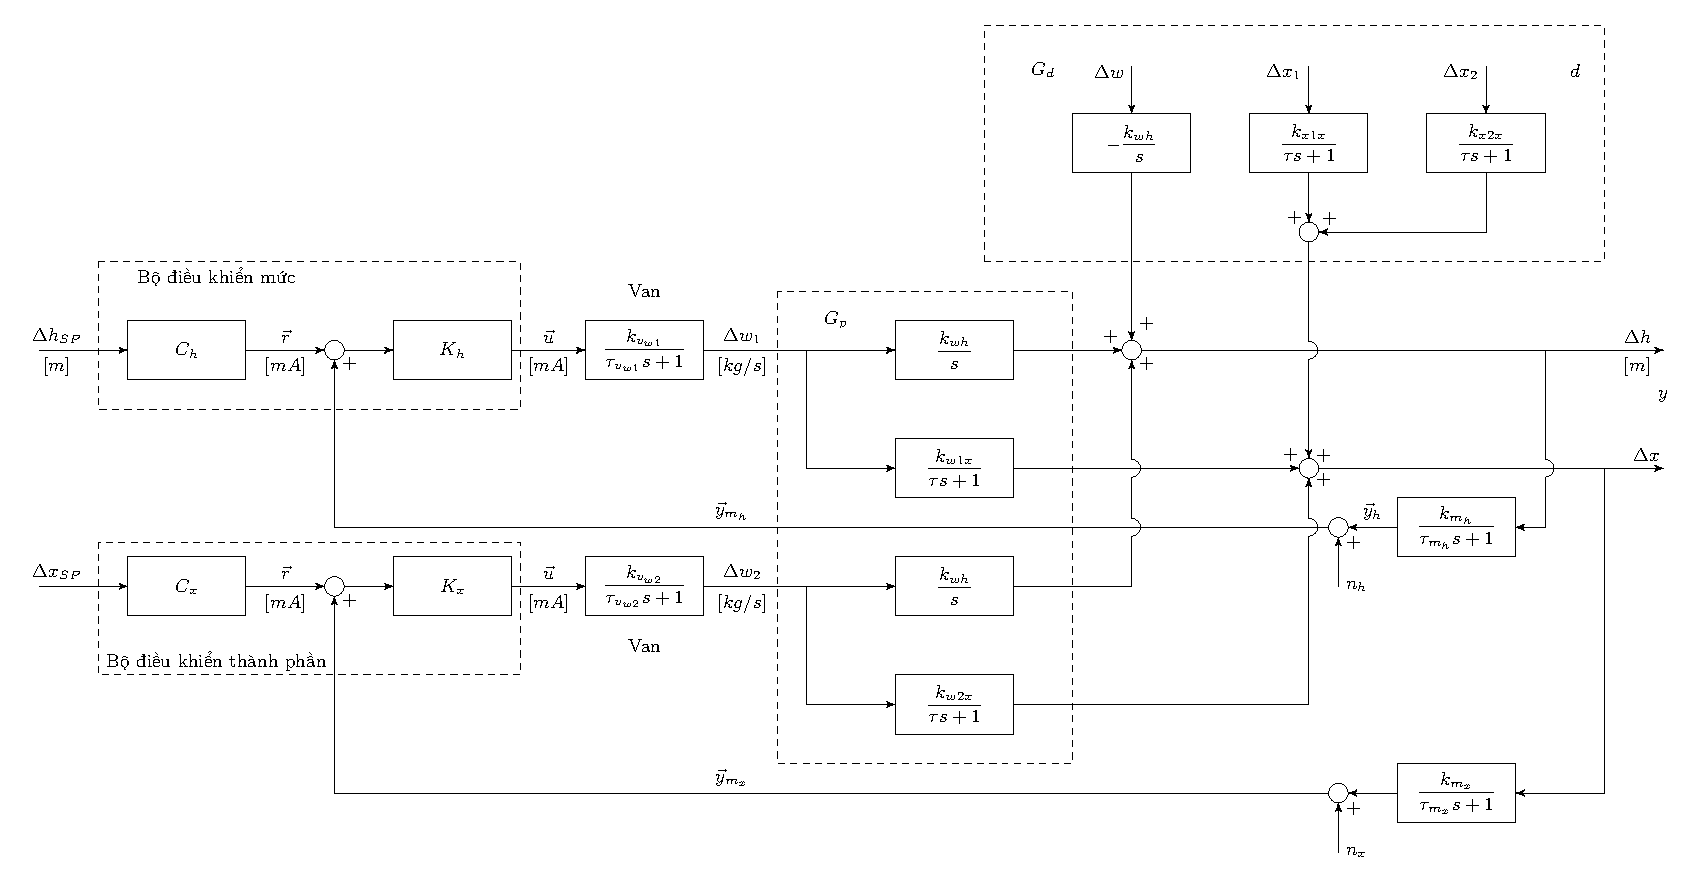
\includegraphics[scale=0.93]{section/mohinhhoalythuyet/images/binhchuachatlong-khuaytron-mohinh1-sodokhoi-cautrucdieukhienphanhoi}
            \end{center}
            \caption{Sơ đồ khối cho cấu trúc điều khiển phản hồi thiết bị khuấy trộn liên tục} \label{Fig:binhchuachatlong-khuaytron-sodokhoi-dieukhienphanhoi}
        \end{figure}
    \end{landscape}

    \subsection{Bài tập về thiết bị khuấy trộn liên tục}
\subsubsection{Mô hình về hai bình chứa chất lỏng nối tiếp nhau}
    \begin{figure}[htp]
        \begin{center}
            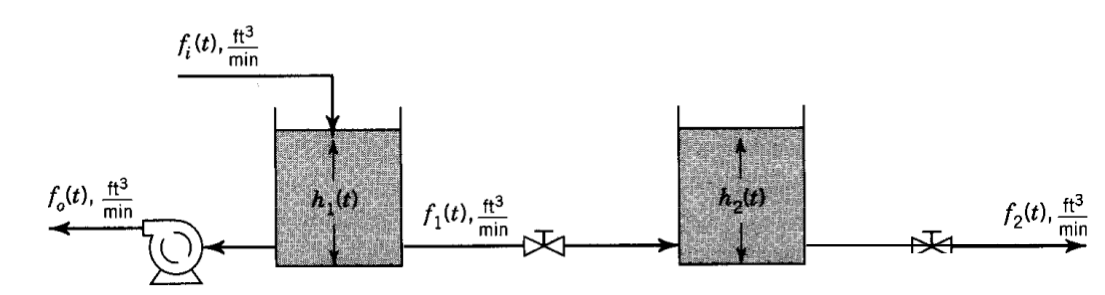
\includegraphics[scale=0.4]{section/mohinhhoalythuyet/images/binhchuachatlong-2binh}
        \end{center}
        \caption{Mô hình về hai bình chứa chất lỏng nối tiếp nhau} \label{Fig:binhchuachatlong-2binh}
    \end{figure}

\subparagraph{Các đại lượng trên mô hình}
    \begin{itemize}
		\item $f_i, f_o, f_1, f_2$: Lưu lượng lưu lượng dòng nguyên liệu $\pfm{ft^3/min}$.
		\item $h_1, h_2$: Mức chất lỏng trong bình $\pfm{m}$.
        \item $A_1, A_2$: Tiết diện của bình chứa $\pfm{m^2}$.
        \item Giả sử đặc tính qua van tuyến tính và lưu lượng qua van được xác định bằng công thức sau: $F = C_v \sqrt{\dfrac{\Delta P}{G_f}}$ với $C_v$ là hệ số van $\pfm{ft^3/s.kPa^{\sfrac{1}{2}}}$, $\Delta P$ là độ chêch lệnh áp suất qua van $\pfm{kPa}$ và $G_f$ là trọng lượng riêng của chất lỏng.
	\end{itemize}

\subparagraph{Mô tả quá trình} Duy trì mức chất lỏng trong mỗi bình ở mức $h_1$ và $h_2$.

\subsubsection{Xác định các biến quá trình}
    \begin{center}
        \begin{tabular}{l|l}
            Biến vào: $f_i, f_o, f_1, f_2$ & Biến điều khiển: $f_1, f_2$ \\ \hline
            Biến ra: $h_1, h_2$ & Biến cần điều khiển: $h_1, h_2$\\ \hline
            & Biến nhiễu: $f_1, f_o$
        \end{tabular}
    \end{center}

\subsubsection{Xây dựng phương trình toán học}
    \begin{itemize}
        \item Xác định lưu lượng dòng chảy qua mỗi van:
            \begin{itemize}
                \item Van 1, ta có: $\Delta P = \pfm{\rho g h_1 + P_a} - \pfm{\rho g h_2 + P_a} = \rho g h_1 - \rho g h_2 = \rho g \pfm{h_1 - h_2}$, nên: $f_1 = C_{v_1} \sqrt{\dfrac{\Delta P}{G_f}} = C_{v_2} \sqrt{\dfrac{\rho g \pfm{h_1 - h_2}}{G_f}} = C_{v_1}^{*}\sqrt{h_1 - h_2}$ với $C_{v_1}^{*} = C_{v_1} \sqrt{\dfrac{\rho g}{G_f}}$.
                \item Van 2, ta có: $\Delta P = \pfm{\rho g h_2 + P_a} - P_a = \rho g h_2$, nên: $f_2 = C_{v_2} \sqrt{\dfrac{\Delta P}{G_f}} = C_{v_2} \sqrt{\dfrac{\rho g h_2}{G_f}} = C_{v_2}^{*}\sqrt{h_2}$ với $C_{v_2}^{*} = C_{v_2} \sqrt{\dfrac{\rho g}{G_f}}$.
            \end{itemize}
        \item Công thức tính thể tích $V = Ah$ với $A$ là tiết diện của bình chứa.
        \item Áp dụng phương trình cân bằng vật chất cho bình chứa 1:
            \begin{align*}
                \dfrac{dV_1}{dt} = f_i - \pfm{f_o + f_1} \Longleftrightarrow \dfrac{d\pfm{A_1 h_1}}{dt} = f_i - f_o - f_1 \Longleftrightarrow \dfrac{dh_1}{dt} = \dfrac{1}{A_1} \pfm{f_i - f_o - f_1}
            \end{align*}
            \item Áp dụng phương trình cân bằng vật chất cho bình chứa 1:
                \begin{align*}
                    \dfrac{dV_2}{dt} = f_1 - f_2 \Longleftrightarrow \dfrac{d\pfm{A_2 h_2}}{dt} = f_1 - f_2 \Longleftrightarrow \dfrac{dh_2}{dt} = \dfrac{1}{A_2} \pfm{f_1 - f_2}
                \end{align*}
        \item Kết luận, mô hình toán của hệ thống là:
            \begin{align*}
                \left\{\begin{array}{l}
                    \dfrac{dh_1}{dt} = \dfrac{1}{A_1} \pfm{f_i - f_o - f_1}\\ [.5cm]
                    \dfrac{dh_2}{dt} = \dfrac{1}{A_2} \pfm{f_1 - f_2}
                \end{array}\right.
            \end{align*}
        \item Thay $f_1 = C_{v_1}^{*}\sqrt{h_1 - h_2}$ và $f_2 = C_{v_2}^{*}\sqrt{h_2}$ (với $C_{v_1}^{*} = C_{v_1} \sqrt{\dfrac{\rho g}{G_f}}$ và $C_{v_2}^{*} = C_{v_2} \sqrt{\dfrac{\rho g}{G_f}}$), ta có:
            \begin{align*}
                \left\{\begin{array}{l}
                    \dfrac{dh_1}{dt} = \dfrac{1}{A_1} \pfm{f_i - f_o - C_{v_1}^{*}\sqrt{h_1 - h_2}}\\[.5cm]
                    \dfrac{dh_2}{dt} = \dfrac{1}{A_2} \pfm{C_{v_1}^{*}\sqrt{h_1 - h_2} - C_{v_2}^{*}\sqrt{h_2}} \\ [.5cm]
                    C_{v_1}^{*} = C_{v_1} \sqrt{\dfrac{\rho g}{G_f}}; \quad C_{v_2}^{*} = C_{v_2} \sqrt{\dfrac{\rho g}{G_f}}
                \end{array}\right.
            \end{align*}
    \end{itemize}

\subsubsection{Tuyến tính hóa phương trình quanh điểm làm việc cân bằng}
    \begin{itemize}
        \item Đặt: $h_1 = \overline{h}_1 + \Delta h_1$; $h_2 = \overline{h}_2 + \Delta h_2$; $f_i = \overline{f}_i + \Delta f_i$; $f_o = \overline{f}_o + \Delta f_o$.
        \item Tại điểm làm việc cân bằng $(\overline{h}_1, \overline{h}_2, \overline{f}_i, \overline{f}_o)$, ta có:
            \begin{align*}
                \left\{\begin{array}{l}
                    \dfrac{dh_1}{dt} = \dfrac{1}{A_1} \pfm{\overline{f}_i - \overline{f}_o - C_{v_1}^{*}\sqrt{\overline{h}_1 - \overline{h}_2}} = 0\\[.5cm]
                    \dfrac{dh_2}{dt} = \dfrac{1}{A_2} \pfm{C_{v_1}^{*}\sqrt{\overline{h}_1 - \overline{h}_2} - C_{v_2}^{*}\sqrt{\overline{h}_2}} = 0\\ [.5cm]
                \end{array}\right.
                \Longleftrightarrow
                \left\{\begin{array}{l}
                     \overline{f}_i - \overline{f}_o - C_{v_1}^{*}\sqrt{\overline{h}_1 - \overline{h}_2} = 0 \\ [.5cm]
                    C_{v_1}^{*}\sqrt{\overline{h}_1 - \overline{h}_2} - C_{v_2}^{*}\sqrt{\overline{h}_2} = 0
                \end{array}\right.
            \end{align*}
        \item Khai triển Taylor cho $f(f_i, f_o, h_1, h_2) = \dfrac{dh_1}{dt} = \dfrac{1}{A_1} \pfm{f_i - f_o - C_{v_1}^{*}\sqrt{h_1 - h_2}}$ tại điểm làm việc cân bằng $(\overline{h}_1, \overline{h}_2, \overline{f}_i, \overline{f}_o)$:
            \begin{align*}
                \dot{h_1} = \Delta \dot{h_1} = & \underbrace{f(\overline{h}_1, \overline{h}_2, \overline{f}_i, \overline{f}_o)}_{0} + \dfrac{df}{df_i}\Delta f_i + \dfrac{df}{df_o}\Delta f_0 + \dfrac{df}{dh_1}\Delta h_1 + \dfrac{df}{dh_2}\Delta h_2 \\
                & = \dfrac{1}{A_1} \pfs{\Delta f_i - \Delta f_o - \dfrac{C_{v_1}^{*}}{2\sqrt{\overline{h}_1 - \overline{h}_2}} \Delta h_1 + \dfrac{C_{v_1}^{*}}{2\sqrt{\overline{h}_1 - \overline{h}_2}} \Delta h_2}
            \end{align*}
        \item Khai triển Taylor cho $g(f_i, f_o, h_1, h_2) = \dfrac{dh_2}{dt} = \dfrac{1}{A_2} \pfm{C_{v_1}^{*}\sqrt{h_1 - h_2} - C_{v_2}^{*}\sqrt{h_2}}$ tại điểm làm việc cân bằng $(f_i, f_o, h_1, h_2)$, ta có:
            \begin{align*}
                \dot{h_2} = \Delta \dot{h_2} = & \underbrace{g(\overline{h}_1, \overline{h}_2, \overline{f}_i, \overline{f}_o)}_{0} + \dfrac{dg}{df_i}\Delta f_i + \dfrac{dg}{df_o}\Delta f_0 + \dfrac{dg}{dh_1}\Delta h_1 + \dfrac{dg}{dh_2}\Delta h_2 \\
                & = \dfrac{1}{A_2} \pfs{\dfrac{C_{v_1}^{*}}{2\sqrt{\overline{h}_1 - \overline{h}_2}} \Delta h_1 - \dfrac{C_{v_1}^{*}}{2\sqrt{\overline{h}_1 - \overline{h}_2}} \Delta h_2 - \dfrac{C_{v_2}^{*}}{2\sqrt{\overline{h}_2}} \Delta h_2}
            \end{align*}
        \item Kết luận, mô hình tuyến tính hóa theo khai triển Taylor có dạng:
            \begin{align*}
                \left\{\begin{array}{l}
                    \Delta \dot{h_1} = \dfrac{1}{A_1} \pfs{\Delta f_i - \Delta f_o - \dfrac{C_{v_1}^{*}}{2\sqrt{\overline{h}_1 - \overline{h}_2}} \Delta h_1 + \dfrac{C_{v_1}^{*}}{2\sqrt{\overline{h}_1 - \overline{h}_2}} \Delta h_2}\\ [.5cm]
                    \Delta \dot{h_2} = \dfrac{1}{A_2} \pfs{\dfrac{C_{v_1}^{*}}{2\sqrt{\overline{h}_1 - \overline{h}_2}} \Delta h_1 - \dfrac{C_{v_1}^{*}}{2\sqrt{\overline{h}_1 - \overline{h}_2}} \Delta h_2 - \dfrac{C_{v_2}^{*}}{2\sqrt{\overline{h}_2}} \Delta h_2}
                \end{array}\right.
            \end{align*}
    \end{itemize}

\subsubsection{Xây dựng hàm truyền và vẽ sơ đồ khối mô tả quá trình}
    \begin{itemize}
        \item Ta có $\Delta \dot{h_1} = \dfrac{1}{A_1} \pfs{\Delta f_i - \Delta f_o - \dfrac{C_{v_1}^{*}}{2\sqrt{\overline{h}_1 - \overline{h}_2}} \Delta h_1 + \dfrac{C_{v_1}^{*}}{2\sqrt{\overline{h}_1 - \overline{h}_2}} \Delta h_2}$, khai triển Laplace:
            \begin{align*}
                & s \Delta H_1(s) = \dfrac{1}{A_1} \pfs{\Delta F_i(s) - \Delta F_o (s) - \dfrac{C_{v_1}^{*}}{2\sqrt{\overline{h}_1 - \overline{h}_2}} \Delta H_1(s) + \dfrac{C_{v_1}^{*}}{2\sqrt{\overline{h}_1 - \overline{h}_2}} \Delta H_2(s)}\\
                \Longleftrightarrow & A_1 s \Delta H_1(s) + \dfrac{C_{v_1}^{*}}{2\sqrt{\overline{h}_1 - \overline{h}_2}} \Delta H_1(s) = \Delta F_i(s) - \Delta F_o (s) + \dfrac{C_{v_1}^{*}}{2\sqrt{\overline{h}_1 - \overline{h}_2}} \Delta H_2(s) \\
                \Longleftrightarrow & \dfrac{A_1}{\dfrac{C_{v_1}^{*}}{2\sqrt{\overline{h}_1 - \overline{h}_2}}} s \Delta H_1(s) + \Delta H_1(s) = \dfrac{1} {\dfrac{C_{v_1}^{*}}{2\sqrt{\overline{h}_1 - \overline{h}_2}}} \Delta F_i(s) - \dfrac{1} {\dfrac{C_{v_1}^{*}}{2\sqrt{\overline{h}_1 - \overline{h}_2}}} \Delta F_o (s) + \Delta H_2(s) \\
                \Longleftrightarrow & \pfm{\dfrac{A_1}{\dfrac{C_{v_1}^{*}}{2\sqrt{\overline{h}_1 - \overline{h}_2}}} s + 1}\Delta H_1(s) = \dfrac{1} {\dfrac{C_{v_1}^{*}}{2\sqrt{\overline{h}_1 - \overline{h}_2}}} \Delta F_i(s) - \dfrac{1} {\dfrac{C_{v_1}^{*}}{2\sqrt{\overline{h}_1 - \overline{h}_2}}} \Delta F_o (s) + \Delta H_2(s)
            \end{align*}
        \item Đặt $m_{h_1} = \dfrac{C_{v_1}^{*}}{2\sqrt{\overline{h}_1 - \overline{h}_2}}$, ta có:
            \begin{align*}
                & \pfm{\dfrac{A_1}{m_{h_1}} s + 1}\Delta H_1(s) = \dfrac{1} {m_{h_1}} \Delta F_i(s) - \dfrac{1}{m_{h_1}} \Delta F_o (s) + \Delta H_2(s) \\
                \Longleftrightarrow & \Delta H_1(s) = \dfrac{\dfrac{1} {m_{h_1}}}{\dfrac{A_1}{m_{h_1}} s + 1} \Delta F_i(s) - \dfrac{\dfrac{1}{m_{h_1}}}{\dfrac{A_1}{m_{h_1}} s + 1} \Delta F_o (s) + \dfrac{1}{\dfrac{A_1}{m_{h_1}} s + 1}\Delta H_2(s)
            \end{align*}
        \item Đặt $k_{h_1} = \dfrac{1}{m_{h_1}}$ và $\tau_{h_1} = \dfrac{A_1}{m_{h_1}}$, ta có:
            \begin{align*}
                \Delta H_1(s) = \dfrac{k_{h_1}}{\tau_{h_1} s + 1} \Delta F_i(s) - \dfrac{k_{h_1}}{\tau_{h_1} s + 1} \Delta F_o (s) + \dfrac{1}{\tau_{h_1} s + 1}\Delta H_2(s)
            \end{align*}
        \item Ta có $\Delta \dot{h_2} = \dfrac{1}{A_2} \pfs{\dfrac{C_{v_1}^{*}}{2\sqrt{\overline{h}_1 - \overline{h}_2}} \Delta h_1 - \dfrac{C_{v_1}^{*}}{2\sqrt{\overline{h}_1 - \overline{h}_2}} \Delta h_2 - \dfrac{C_{v_2}^{*}}{2\sqrt{\overline{h}_2}} \Delta h_2}$, khai triển Laplace:
            \begin{align*}
                & s H_2(s) = \dfrac{1}{A_2} \pfs{\dfrac{C_{v_1}^{*}}{2\sqrt{\overline{h}_1 - \overline{h}_2}} \Delta H_1(s) - \dfrac{C_{v_1}^{*}}{2\sqrt{\overline{h}_1 - \overline{h}_2}} \Delta H_2(s) - \dfrac{C_{v_2}^{*}}{2\sqrt{\overline{h}_2}} \Delta H_2(s)}\\
                \Longleftrightarrow & A_2 s \Delta H_2(s) + \dfrac{C_{v_2}^{*}}{2\sqrt{\overline{h}_2}} \Delta H_2(s) + \dfrac{C_{v_1}^{*}}{2\sqrt{\overline{h}_1 - \overline{h}_2}} \Delta H_2(s)= \dfrac{C_{v_1}^{*}}{2\sqrt{\overline{h}_1 - \overline{h}_2}} \Delta H_1(s) \\
                \Longleftrightarrow & \pfm{A_2 s + \dfrac{C_{v_2}^{*}}{2\sqrt{\overline{h}_2}} + \dfrac{C_{v_1}^{*}}{2\sqrt{\overline{h}_1 - \overline{h}_2}}} \Delta H_2(s)= \dfrac{C_{v_1}^{*}}{2\sqrt{\overline{h}_1 - \overline{h}_2}} \Delta H_1(s) \\
                \Longleftrightarrow & \pfm{\dfrac{A_2}{\dfrac{C_{v_2}^{*}}{2\sqrt{\overline{h}_2}} + \dfrac{C_{v_1}^{*}}{2\sqrt{\overline{h}_1 - \overline{h}_2}}}s + 1} \Delta H_2(s)= \dfrac{\dfrac{C_{v_1}^{*}}{2\sqrt{\overline{h}_1 - \overline{h}_2}}}{\dfrac{C_{v_2}^{*}}{2\sqrt{\overline{h}_2}} + \dfrac{C_{v_1}^{*}}{2\sqrt{\overline{h}_1 - \overline{h}_2}}} \Delta H_1(s)
            \end{align*}
        \item Đặt $m_{h_2} = \dfrac{C_{v_2}^{*}}{2\sqrt{\overline{h}_2}} + \dfrac{C_{v_1}^{*}}{2\sqrt{\overline{h}_1 - \overline{h}_2}}$, ta có:
            \begin{align*}
                \pfm{\dfrac{A_2}{m_{h_2}}s + 1} \Delta H_2(s)= \dfrac{\dfrac{C_{v_1}^{*}}{2\sqrt{\overline{h}_1 - \overline{h}_2}}}{m_{h_2}} \Delta H_1(s)
            \end{align*}
        \item Đặt $\tau_{h_2} = \dfrac{A_2}{m_{h_2}}$ và $k_{h_2} = \dfrac{\dfrac{C_{v_1}^{*}}{2\sqrt{\overline{h}_1 - \overline{h}_2}}}{m_{h_2}}$, ta có:
            \begin{align*}
                \pfm{\tau_{h_2}s + 1} \Delta H_2(s) = k_{h_2} \Delta H_1(s) \Longleftrightarrow \Delta H_2(s) = \dfrac{k_{h_2}}{\tau_{h_2}s + 1} \Delta H_1(s) \Longleftrightarrow H_1(s) = \dfrac{\tau_{h_2}s + 1}{k_{h_2}}
            \end{align*}
        \item Ta có:
            \begin{align*}
                \left\{\begin{array}{l}
                    \Delta H_1(s) = \dfrac{k_{h_1}}{\tau_{h_1} s + 1} \Delta F_i(s) - \dfrac{k_{h_1}}{\tau_{h_1} s + 1} \Delta F_o (s) + \dfrac{1}{\tau_{h_1} s + 1}\Delta H_2(s) \\ [.5cm]
                    \Delta H_1(s) = \dfrac{\tau_{h_2}s + 1}{k_{h_2}} \Delta H_2(s)
                \end{array}\right.
            \end{align*}
        \item Suy ra:
            \begin{align*}
                & \dfrac{\tau_{h_2}s + 1}{k_{h_2}} \Delta H_2(s) = \dfrac{k_{h_1}}{\tau_{h_1} s + 1} \Delta F_i(s) - \dfrac{k_{h_1}}{\tau_{h_1} s + 1} \Delta F_o (s) + \dfrac{1}{\tau_{h_1} s + 1}\Delta H_2(s) \\
                \Longleftrightarrow & \pfm{\dfrac{\tau_{h_2}s + 1}{k_{h_2}} - \dfrac{1}{\tau_{h_1} s + 1}} \Delta H_2(s) = \dfrac{k_{h_1}}{\tau_{h_1} s + 1} \Delta F_i(s) - \dfrac{k_{h_1}}{\tau_{h_1} s + 1} \Delta F_o (s) \\
                \Longleftrightarrow & \pfs{\dfrac{\pfm{\tau_{h_2}s + 1}\pfm{\tau_{h_1} s + 1} - k_{h_2}}{k_{h_2}\pfm{\tau_{h_1} s + 1}}} \Delta H_2(s) = \dfrac{k_{h_1}}{\tau_{h_1} s + 1} \Delta F_i(s) - \dfrac{k_{h_1}}{\tau_{h_1} s + 1} \Delta F_o (s) \\
                \Longleftrightarrow & \pfs{\pfm{\tau_{h_2}s + 1}\pfm{\tau_{h_1} s + 1} - k_{h_2}} \Delta H_2(s) = k_{h_1} k_{h_2} F_i(s) - k_{h_1} k_{h_2} F_o(s) \\
                \Longleftrightarrow & \Delta H_2(s) = \frac{k_{h_1} k_{h_2}}{\pfm{\tau_{h_2}s + 1}\pfm{\tau_{h_1} s + 1} - k_{h_2}} F_i(s) - \frac{k_{h_1} k_{h_2}}{\pfm{\tau_{h_2}s + 1}\pfm{\tau_{h_1} s + 1} - k_{h_2}} F_o(s)
            \end{align*}
        \item Kết luận:
            \begin{align*}
                \left\{\begin{array}{l}
                    \dfrac{H_2(s)}{F_i(s)} = \frac{k_{h_1} k_{h_2}}{\pfm{\tau_{h_2}s + 1}\pfm{\tau_{h_1} s + 1} - k_{h_2}}; \quad \dfrac{H_2(s)}{F_o(s)} = -\frac{k_{h_1} k_{h_2}}{\pfm{\tau_{h_2}s + 1}\pfm{\tau_{h_1} s + 1} - k_{h_2}}
                \end{array}\right.
            \end{align*}
        \item Sơ đồ khối mô tả quá trình:
            \begin{figure}[htp]
                \begin{center}
                    \subimport{section/mohinhhoalythuyet/images/}{binhchuanoitiep-sodokhoi.tex}
                \end{center}
                \caption{Sơ đồ khối mô tả quá trình} \label{Fig:binhchuanoitiep-sodokhoi}
            \end{figure}
    \end{itemize}

\subsubsection{Vẽ sơ đồ khối cho cấu trúc điều khiển phản hồi}
    % \begin{landscape}
    %     \begin{figure}[htp]
    %         \begin{center}
    %             \subfloat[Mô hình 1 \label{Fig:binhchuachatlong-khuaytron-mohinh1}]
    %                 {
    %                     %\subimport{section/mohinhhoalythuyet/images/}{binhchuachatlong-khuaytron-mohinh1-sodokhoi-cautrucdieukhienphanhoi.tex}
    %                     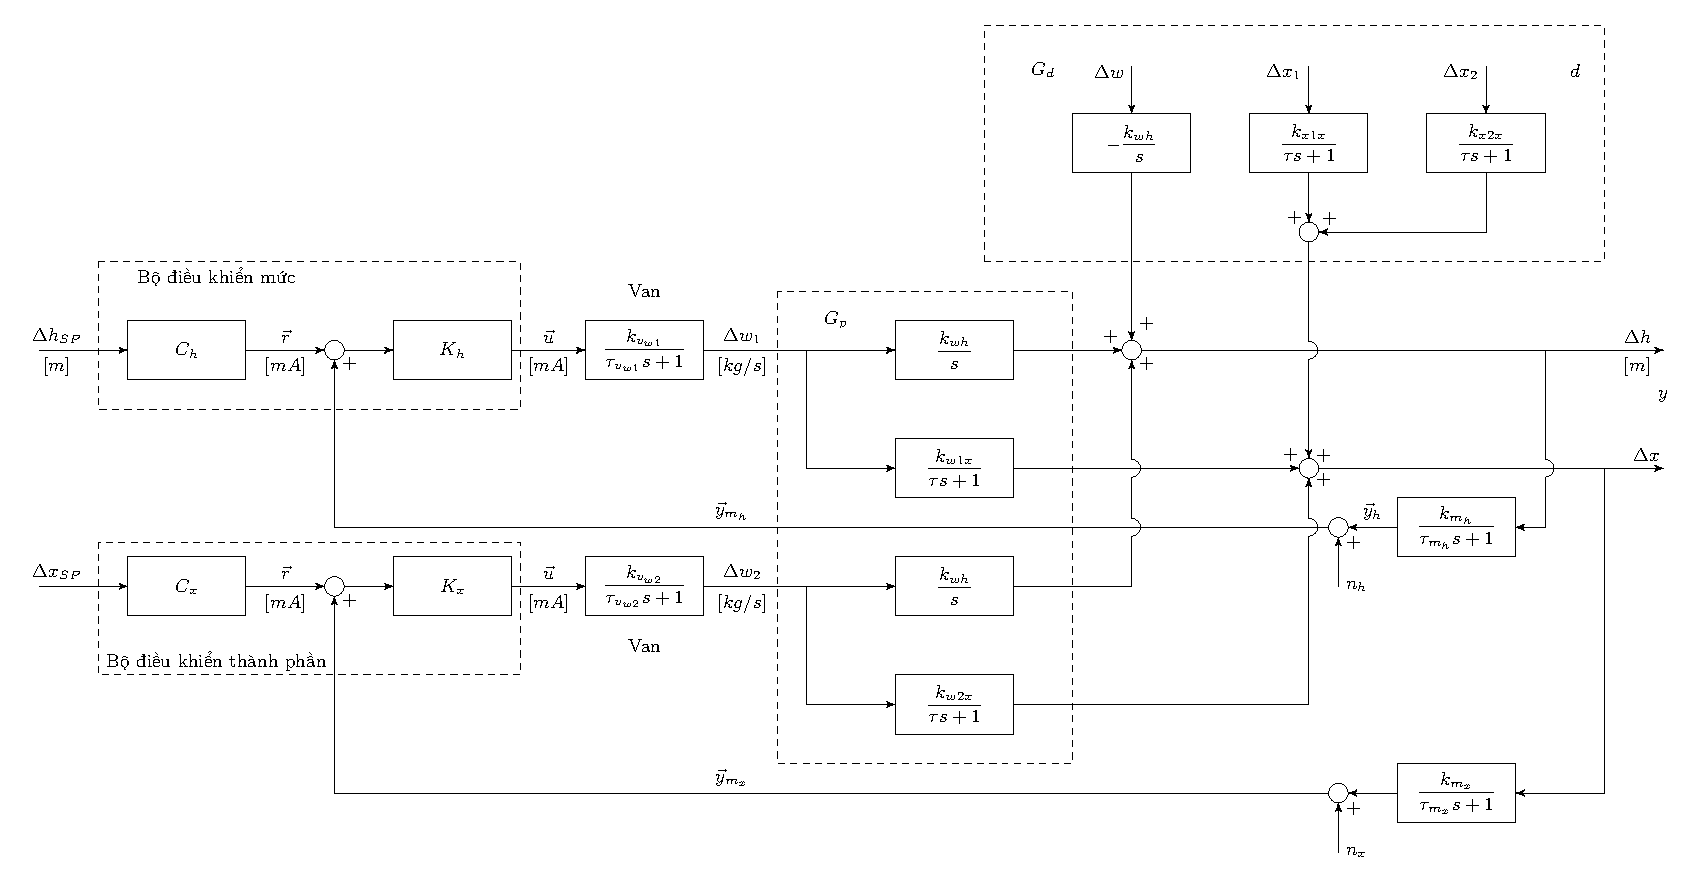
\includegraphics[scale=0.93]{section/mohinhhoalythuyet/images/binhchuachatlong-khuaytron-mohinh1-sodokhoi-cautrucdieukhienphanhoi}
    %                 }
    %         \end{center}
    %         \caption{Sơ đồ khối cho cấu trúc điều khiển phản hồi thiết bị khuấy trộn liên tục} \label{Fig:binhchuachatlong-khuaytron-sodokhoi-dieukhienphanhoi}
    %     \end{figure}
    % \end{landscape}



\end{document}
